\chapter*{Wprowadzenie}
\addcontentsline{toc}{chapter}{Wprowadzenie}
\label{cha:wstep}


\begin{figure}[h]
\centering
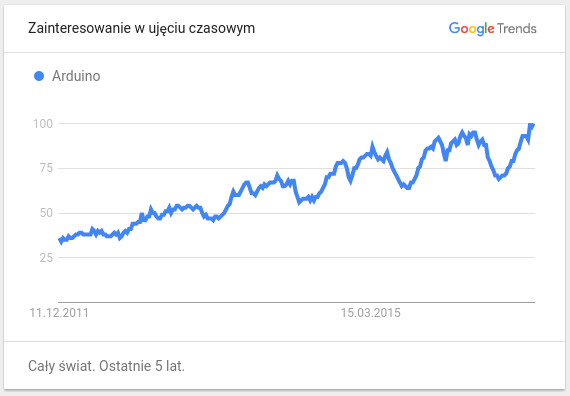
\includegraphics[width=0.7\textwidth]{images/arduino-trends.png}
\caption{Relatywna liczba wyszukiwań frazy ,,Arduino'' w ostatnich pięciu latach. Źródło: Google Trends}
\label{fig:arduinotrends}
\end{figure}

AVR to rodzina mikroprocesorów opracowana i rozwijana przez firmę Atmel. Oparta o nią jest m. in. platforma Arduino, która -- jak przedstawiono na Rys. \ref{fig:arduinotrends} -- z roku na rok zyskuje popularność. Platforma Arduino zaprojektowana została z myślą o osobach, które niekoniecznie posiadają formalne wykształcenie inżynierskie~\cite{BanShi14}. Jest ona też często używana do prototypowania urządzeń, wpisujących się w koncepcję \emph{Internetu Rzeczy (ang. \gls{iot})}.

Urządzenia wbudowane podłączone do Internetu są szczególnie narażone na ataki. W 2016 roku podatne urządzenia wbudowane zostały wykorzystane do przeprowadzenia masywnych ataków typu \gls{ddos}~\cite{AkaIOT}.

Istotne jest więc dostarczenie narzędzi, które pozwalają nie tylko na szybkie prototypowanie, ale które pozwolą także zachować odpowiedni poziom bezpieczeństwa. Należy pamiętać przede wszystkim o tym, że urządzenia \emph{IoT} są tworzone także przez ludzi bez formalnego wykształcenia inżynierskiego.

W niniejszej pracy przedstawiono protokół bezpiecznej komunikacji oraz bibliotekę programistyczną na urządzenia AVR zaprojektowane z myślą o prostocie obsługi. Wybrane zostały zestawy algorytmów, które zapewniają niezbędny poziom bezpieczeństwa. Ich złożoność została ukryta za prostym interfejsem programistycznym \emph{(ang. \acrshort{iot})}, który nie pozwala na wprowadzenie błędów zmniejszających bezpieczeństwo.  Zaproponowane rozwiązanie zapewnia poufność, autentyczność oraz integralność przesyłanych danych.

W rozdziale \ref{cha:hardware} scharakteryzowana jest platforma sprzętowa AVR, ze szczególnym uwzględnieniem jej ograniczeń. Następnie w rozdziale \ref{cha:metodyUwierzytelniania} przedstawione zostały różne metody uwierzytelniania i uzasadniony został wybór konkretnych rozwiązań. Implementacja została szczegółowo opisana w rozdziale \ref{cha:implementacja}. Całość rozwiązania została zwalidowana poprzez porównanie z implementacją na inną platformę, co opisano w rozdziale \ref{cha:walidacja}. W rozdziale \ref{cha:podsumowanie} podsumowano całe rozwiązanie oraz przedstawiono jego ograniczenia i słabe strony.

Całość kodu źródłowego dostępna jest w serwisie GitHub\footnote{\url{https://github.com/kacperzuk/seconn}}.
